\begin{frame}{$V$-Tree}
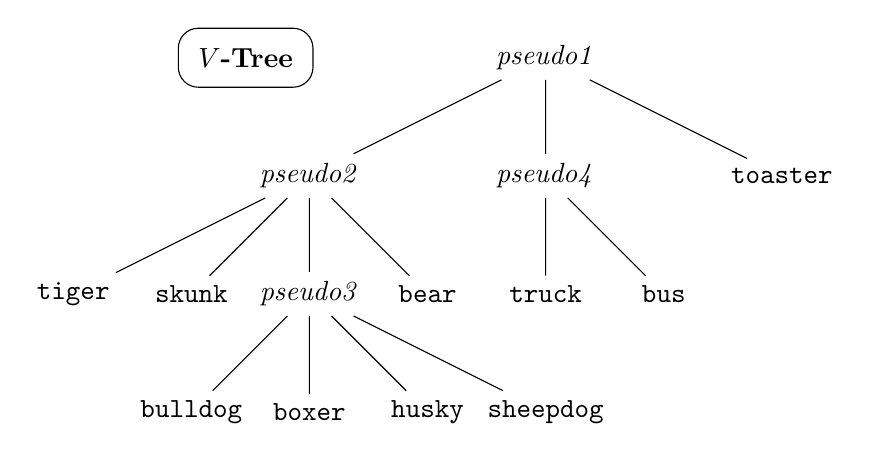
\begin{tikzpicture}
    [ level distance=1.5cm
    , level 1/.style={sibling distance=3cm}
    , level 2/.style={sibling distance=1.5cm}
    ]
\node[draw, rounded corners=0.1in, inner sep=0.1in] at (-1.5in,0){\textbf{$V$-Tree}};
\node {\textit{pseudo1}}
    child {node {\textit{pseudo2}}
      child {node {\texttt{tiger}}}
      child {node {\texttt{skunk}}}
      child {node {\textit{pseudo3}}
        child {edge from parent[draw=none]} % Added
        child {node {\texttt{bulldog}}}
        child {node {\texttt{boxer}}}
        child {node {\texttt{husky}}}
        child {node {\texttt{sheepdog}}}
      }
      child {node {\texttt{bear}}}
      child {edge from parent[draw=none]} % Added
      }
    child {node {\textit{pseudo4}}
      child {edge from parent[draw=none]} % Added
      child {node {\texttt{truck}}}
      child {node {\texttt{bus}}}
    }
    child {node {\texttt{toaster}}}
    ;

\end{tikzpicture}
\end{frame}
